\setcounter{chapter}{4}
\chapter{Appendix:線形代数}
%
講義では触れないが,
線形代数は今後化学工学を学び,研究活動を行う上で役に立つことが多い.
そこで,本章では線形代数について簡単にまとめておく.
%
\section{行列とベクトル}
%
ここでは,行列についての基本的事項について述べる.
既によく理解している人は次の節から読み進めても問題ない.
%
\subsection{行列の表し方}
%
行列とは数を縦方向(行)・横方向(列)に並べたものを指す.また,行列を数と区別するために,$\hat{}$ (ハット)をつけて$\hat{A}$のように表すことにする\footnote{行列の表し方は教科書によって異なる.} .
行列の例を以下に2つ示しておく.
\begin{align}
\hat{A} & =\begin{array}{cc}
\text{列}\\
\left[\begin{array}{cc}
1 & 2\\
3 & 4
\end{array}\right] & \text{行}\\
\\
\end{array},\\
\hat{B} &=\left[\begin{array}{ccc}
4 & 10 & 2\\
1 & 4 & 9\\
5 & 3 & 7\\
8 & 6 & 2
\end{array}\right], 
\end{align}

行列$\hat{A}$の第$i$行,第$j$列の成分を$(i,j)$成分と呼び,
その成分の値を$A_{ij}$と表すことにする.
$m$行$n$列の行列を$m\times n$型の行列,
またはもっと略して$m\times n$行列と表すことが一般的である.上の例では,
$\hat{A}$は$2\times 2$行列,$\hat{B}$は$4\times 3$行列である.
%
さらに,$(i,j)$成分が$A_{ij}$の$m\times n$行列を
\begin{align}
 \hat{A} & =\left[A_{ij}\right]_{m\times n},
\end{align}
のように表すこととする.
%
%
\subsection{転置(transpose)}
%
行列$\hat{A}$の転置(transpose)行列とは,行列の縦横を入れ替えたものを指し,
$^{t}\hat{A}$のように,左上に$t$をつけて表す.
上の例では,
\begin{align}
 ^{t}\hat{A} & =\left[\begin{array}{cc}
1 & 3\\
2 & 4
\end{array}\right] 
\end{align}
である.また,成分表示で表すと,
\begin{align}
^{t}A_{ij} & =A_{ji},
\end{align}
である.
%
\subsection{縦(列)ベクトルと横(行)ベクトル\label{sec:row-column_vector}}
%
$m\times 1$行列のことを$m$成分の縦(列)ベクトルと呼ぶ.縦ベクトルは例えば次の${\bf u}$のようなものである.
\begin{align}
 {\bf u} & =\left[\begin{array}{c}
2\\
1\\
3
\end{array}\right], 
\end{align}
このようにベクトルも行列の1種と見做すことができる.
このテキストでは,ベクトルの場合は区別のため$\hat{u}$ではなく${\bf v}$のようにボールドで表すことにする.
%
同様に,$1\times n$行列のことを$n$成分の横(行)ベクトルと呼ぶ.例えば,以下の${\bf v}$は行ベクトルである.
\begin{align}
{\bf v} & =\left[\begin{array}{ccc}
4 & 2 & 5\end{array}\right]  
\end{align}
縦ベクトルから横ベクトル,また横ベクトルから縦ベクトルへの
変換は,転置をとることに対応する.
\begin{align}
 ^{t}{\bf v} & = {}^{t}\left[\begin{array}{ccc}
4 & 2 & 5\end{array}\right]\notag\\
 & =\left[\begin{array}{c}
4\\
2\\
5
\end{array}\right]. 
\end{align}
%

$m\times n$行列をベクトルの集まりと見做すこともできる.
%
$m$成分の縦ベクトル${\bf u}_{1},~{\bf u}_{2},\cdots,{\bf u}_{n}$を考え,
${\bf u}_{j}$の$(i,1)$成分(つまり第$i$成分)を$u_{ij}$と書くことにする.
\begin{align}
{\bf u}_{j} & =\left[\begin{array}{c}
u_{1j}\\
u_{2j}\\
\vdots\\
u_{ij}\\
\vdots\\
u_{mj}
\end{array}\right].  
\end{align}
この$n$個の縦ベクトルを横に並べた行列を$\hat{U}$とすると,
\begin{align}
\hat{U} & =\left[\begin{array}{cccccc}
{\bf u}_{1} & {\bf u}_{2} & \cdots & {\bf u}_{j} & \cdots & {\bf u}_{n}\end{array}\right]\notag\\
 & =\left[\begin{array}{cccccc}
u_{11} & u_{12} & \cdots & u_{1j} & \cdots & u_{1n}\\
u_{21} & u_{22} & \cdots & u_{2j} & \cdots & u_{2n}\\
\vdots & \vdots & \ddots & \vdots &  & \vdots\\
u_{i1} & u_{i2} & \cdots & u_{ij} & \cdots & u_{in}\\
\vdots & \vdots &  & \vdots & \ddots & \vdots\\
u_{m1} & u_{m2} & \cdots & u_{mj} & \cdots & u_{mn}
\end{array}\right],
\end{align}
となる.つまり,$\hat{U}=\left[u_{ij}\right]_{m\times n}$を$n$個の縦ベクトルの集まりで表せた,ということになる.
同様に行列を縦ベクトルの集まりで表すこともできる.
$n$成分の横ベクトル${\bf v}_{1},~{\bf v}_{2},\cdots,~{\bf v}_{m}$ (${\bf v}_{i}$の$(1,j)$成分を$v_{ij}$とする)
を縦に並べた行列$\hat{V}$は
\begin{align}
\hat{V} & =\left[\begin{array}{c}
{\bf v}_{1}\\
{\bf v}_{2}\\
\vdots\\
{\bf v}_{i}\\
\vdots\\
{\bf v}_{m}
\end{array}\right]=\left[\begin{array}{cccccc}
v_{11} & v_{12} & \cdots & v_{1j} & \cdots & v_{1n}\\
v_{21} & v_{22} & \cdots & v_{2j} & \cdots & v_{2n}\\
\vdots & \vdots & \ddots & \vdots &  & \vdots\\
v_{i1} & v_{i2} & \cdots & v_{ij} & \cdots & v_{in}\\
\vdots & \vdots &  & \vdots & \ddots & \vdots\\
v_{m1} & v_{m2} & \cdots & v_{mj} & \cdots & v_{mn}
\end{array}\right], 
\end{align}
となり,これは$m\times n$の行列$\hat{V}=\left[v_{ij}\right]_{m\times n}$である.
行列を縦ベクトルや横ベクトルの集まりと考えるという視点は,線形代数やその応用を学ぶ上で重要である.
%
%
\subsection{行列の演算\label{sec:mat_operation}}
%
\begin{itemize}
\item \textbf{和と差}\\
%
2つの行列$\hat{A},~\hat{B}$の型が同じであれば,
行列の和や差を定義することできる.
ここでは,$\hat{A},~\hat{B}$を$2\times 2$行列とする.
%
\begin{align}
\hat{A} & =\left[\begin{array}{cc}
a & b\\
c & d
\end{array}\right],\quad\hat{B}=\left[\begin{array}{cc}
a^{\prime} & b^{\prime}\\
c^{\prime} & d^{\prime}
\end{array}\right].
\end{align}
%
行列の和$\hat{A}+\hat{B}$とは2つの行列の各成分の和をとったもののことを指す.
上の$\hat{A},~\hat{B}$を使って例示すると,
%
\begin{align}
\hat{A}+\hat{B} & =\left[\begin{array}{cc}
a & b\\
c & d
\end{array}\right]+\left[\begin{array}{cc}
a^{\prime} & b^{\prime}\\
c^{\prime} & d^{\prime}
\end{array}\right]\notag\\
 & =\left[\begin{array}{cc}
a+a^{\prime} & b+b^{\prime}\\
c+c^{\prime} & d+d^{\prime}
\end{array}\right],
\end{align}
である.次に,行列の差について述べる.
%
行列$\hat{B}$の全ての成分に$-1$をかけた行列を$-\hat{B}$のように書くことにする.
つまり,
\begin{align}
-\hat{B} & =-\left[\begin{array}{cc}
a^{\prime} & b^{\prime}\\
c^{\prime} & d^{\prime}
\end{array}\right]=\left[\begin{array}{cc}
-a^{\prime} & -b^{\prime}\\
-c^{\prime} & -d^{\prime}
\end{array}\right], 
\end{align}
である.行列の差$\hat{A}-\hat{B}$を行列$\hat{A}$と$-\hat{B}$の和$\hat{A}+(-\hat{B})$と定義することにする.
%
\begin{align}
\hat{A}-\hat{B} & =\left[\begin{array}{cc}
a & b\\
c & d
\end{array}\right]-\left[\begin{array}{cc}
a^{\prime} & b^{\prime}\\
c^{\prime} & d^{\prime}
\end{array}\right]\notag\\
 & =\left[\begin{array}{cc}
a & b\\
c & d
\end{array}\right]+\left[\begin{array}{cc}
-a^{\prime} & -b^{\prime}\\
-c^{\prime} & -d^{\prime}
\end{array}\right]\notag\\
 & =\left[\begin{array}{cc}
a-a^{\prime} & b-b^{\prime}\\
c-c^{\prime} & d-d^{\prime}
\end{array}\right]. 
\end{align}
%
$m\times n$型の行列$\hat{A}=\left[A_{ij}\right]_{m\times n},~\hat{B}=\left[B_{ij}\right]_{m\times n}$についても
同様に,和と差を定義することができる.例えば,和については次式のようになる.
\begin{align}
\hat{A}+\hat{B} & =\left[\begin{array}{cccc}
A_{11} & A_{12} & \cdots & A_{1n}\\
A_{21} & A_{22} & \cdots\\
\vdots &  & \ddots\\
A_{m1} & \cdots &  & A_{mn}
\end{array}\right]+\left[\begin{array}{cccc}
B_{11} & B_{12} & \cdots & B_{1n}\\
B_{21} & B_{22} & \cdots\\
\vdots &  & \ddots\\
B_{m1} & \cdots &  & B_{mn}
\end{array}\right]\notag\\
 & =\left[\begin{array}{cccc}
A_{11}+B_{11} & A_{12}+B_{12} & \cdots & A_{1n}+B_{1n}\\
A_{21}+B_{21} & A_{22}+B_{22} & \cdots\\
\vdots &  & \ddots\\
A_{m1}+B_{m1} & \cdots &  & A_{mn}+B_{mn}
\end{array}\right]\notag\\
 & =\left[A_{ij}+B_{ij}\right]_{m\times n}. 
\end{align}
%
行列の和や差については,和をとる順序で結果は変わらない.
つまり,$\hat{A},~\hat{B},~\hat{C}$を同じ型の行列とすると次式が成り立つ(すぐに確認できる).
\begin{align}
 \hat{A}+\hat{B} & =\hat{B}+\hat{A},\\
\hat{A}+\left(\hat{B}+\hat{C}\right) & =\left(\hat{A}+\hat{B}\right)+\hat{C},
\end{align}
%
\item \textbf{スカラー倍}\\
%
行列$\hat{A}$の各成分を$k$倍したものを$k\hat{A}$と表す.
\begin{align}
k\hat{A} & =k\left[\begin{array}{cccc}
A_{11} & A_{12} & \cdots & A_{1n}\\
A_{21} & A_{22} & \cdots\\
\vdots &  & \ddots\\
A_{m1} & \cdots &  & A_{mn}
\end{array}\right]=\left[\begin{array}{cccc}
kA_{11} & kA_{12} & \cdots & kA_{1n}\\
kA_{21} & kA_{22} & \cdots\\
\vdots &  & \ddots\\
kA_{m1} & \cdots &  & kA_{mn}
\end{array}\right].
\end{align}
行列やベクトルに数$k$をかけることをスカラー倍と呼ぶ.
スカラー倍は,次の性質を持つ.
\begin{align}
 k\left(l\hat{A}\right) & =kl\hat{A},\\
\left(k+l\right)\hat{A} & =k\hat{A}+l\hat{A},\\
k\left(\hat{A}+\hat{B}\right) & =k\hat{A}+k\hat{B}. 
\end{align}
1つ目の式を結合法則,2つ目と3つ目の式を分配法則と呼ぶ.
%
\item \textbf{行列の積}\\
%
ここでは行列の積を導入する.
%$\hat{A}=\left[A_{ij}\right]_{m\times l}$,$\hat{B}=\left[B_{ij}\right]_{l\times n}$とする.
%$\hat{A}$と$\hat{B}$の積$\hat{A}\hat{B}$によって得られる行列を$\hat{C}$とし,その$(i,j)$成分$C_{ij}$を
%
%\begin{align}
% C_{ij} & =\sum_{k=1}^{l}A_{ik}B_{kj},
%\end{align}
%
%と定めることにする.
%
\Sec{row-column_vector}で述べたように,
行列は列ベクトルや行ベクトルの集まりと考えることができる.
そこで,まずは行ベクトルと列ベクトルの積を定義する.
%
$l$成分の横ベクトル${\bf a}$と$l$成分の縦ベクトル${\bf b}$を考え,
その第$i$成分をそれぞれ$a_{i},~b_{i}$とする.
%
${\bf a}$と${\bf b}$の積を次式で定義する.
%
\begin{align}
{\bf a}{\bf b} & =\left[\begin{array}{ccccc}
a_{1} & \cdots & a_{i} & \cdots & a_{l}\end{array}\right]\left[\begin{array}{c}
b_{1}\\
\vdots\\
b_{i}\\
\vdots\\
b_{l}
\end{array}\right]\notag\\
 & =a_{1}b_{1}+a_{2}b_{2}+\cdots+a_{i}b_{i}+\cdots+a_{l}b_{l}\notag\\
 & =\sum_{i=1}^{l} a_{i}b_{i}. 
\end{align}
%
つまり,縦ベクトルと横ベクトルの積は,各成分の積を足し合わせた量となる.
また,上式の縦ベクトルと横ベクトルの積が考えることができるのは,縦ベクトルと横ベクトルで成分数が一致しているときのみである.

次に,$m$個の横ベクトル${\bf a}_{1},~{\bf a}_{2},\cdots,~{\bf a}_{m}$を縦に並べてできる行列$\hat{A}$
と$n$個の縦ベクトル${\bf b}_{1},~{\bf b}_{2},\cdots,~{\bf b}_{n}$を横に並べてできる行列$\hat{B}$を考える.
ただし,${\bf a}_{i}$, ${\bf b}_{j}$ともに成分数は$l$であるとする.
%
\begin{align}
\hat{A} & =\left[\begin{array}{c}
{\bf a}_{1}\\
\vdots\\
{\bf a}_{i}\\
\vdots\\
{\bf a}_{m}
\end{array}\right]=\left[\begin{array}{cccc}
a_{11} & a_{12} & \cdots & a_{1l}\\
a_{21} & a_{22} &  & a_{2l}\\
\vdots &  & \ddots & \vdots\\
a_{m1} & a_{m2} & \cdots & a_{ml}
\end{array}\right],\\
\hat{B} & =\left[\begin{array}{ccccc}
{\bf b}_{1} & \cdots & {\bf b}_{j} & \cdots & {\bf b}_{n}\end{array}\right]\notag\\
 & =\left[\begin{array}{cccc}
b_{11} & b_{12} & \cdots & b_{1n}\\
b_{21} & b_{22} &  & b_{2n}\\
\vdots &  & \ddots & \vdots\\
b_{l1} & b_{l2} & \cdots & b_{ln}
\end{array}\right].
\end{align}
%
$\hat{A}$は$m\times l$行列,$\hat{B}$は$l\times n$行列である.
2つの行列の積$\hat{A}\hat{B}$を次式で定義する.
%
\begin{align}
\hat{A}\hat{B} & =\left[\begin{array}{cccccc}
{\bf a}_{1}{\bf b}_{1} & {\bf a}_{1}{\bf b}_{2} & \cdots & {\bf a}_{1}{\bf b}_{j} & \cdots & {\bf a}_{1}{\bf b}_{n}\\
{\bf a}_{2}{\bf b}_{1} & {\bf a}_{2}{\bf b}_{2} &  & \vdots &  & \vdots\\
\vdots & \vdots & \ddots & \vdots &  & \vdots\\
{\bf a}_{i}{\bf b}_{1} & {\bf a}_{i}{\bf b}_{2} & \cdots & {\bf a}_{i}{\bf b}_{j} & \cdots & {\bf a}_{i}{\bf b}_{n}\\
\vdots & \vdots &  & \vdots & \ddots & \vdots\\
{\bf a}_{m}{\bf b}_{1} & {\bf a}_{m}{\bf b}_{2} & \cdots & {\bf a}_{m}{\bf b}_{j} & \cdots & {\bf a}_{m}{\bf b}_{n}
\end{array}\right]. 
\end{align}
%
$\hat{C}=\hat{A}\hat{B}$とすると,$\hat{C}$は$m\times n$行列であり,
その$(i,j)$成分$C_{ij}$は
%
\begin{align}
C_{ij} & = {\bf a}_{i}{\bf b}_{j} = \sum_{k=1}^{l}a_{ik}b_{kj},
\end{align}
%
である.行列の積を定められるのは,左側の行列($\hat{A}$)の列数と右側の行列($\hat{B}$)の行数が一致しているときである.
%
\item \textbf{行列の積の性質}\\
%
行列の積について,以下の関係式が成り立つ.
\begin{align}
&k\hat{A}\hat{B}  =\left(k\hat{A}\right)\hat{B}=\hat{A}\left(k\hat{B}\right), \label{LA:matmul_scalar}\\
&\hat{A}\hat{B}\hat{C}  =\left(\hat{A}\hat{B}\right)\hat{C}=\hat{A}\left(\hat{B}\hat{C}\right),\\
&\left(\hat{A}+\hat{B}\right)\hat{C}  =\hat{A}\hat{C}+\hat{B}\hat{C}. \label{LA:matmult_parti} 
\end{align}
ただし,$k$は行列ではなく数である.また,$\hat{A}$の行数と列数が等しい場合($n\times n$行列,正方行列と呼ぶ),$\hat{A}$を$k$回かけたものが定義できる.
これを$\hat{A}^{k}$と表す.
\begin{align}
 \hat{A}^{k}=\underbrace{\hat{A}\hat{A}\cdots \hat{A}}_{k個}. 
\end{align}

これらは数の積の性質と同じである.
その一方で,数の積にはない性質もある.それは行列の積$\hat{A}\hat{B}$と$\hat{B}\hat{A}$が
特別な場合を除いて一致しないということである.
%
$\hat{A}\hat{B}=\hat{B}\hat{A}$が成り立つとき,$\hat{A}$と$\hat{B}$は可換であるといい,
$\hat{A}\hat{B}\neq \hat{B}\hat{A}$のとき,$\hat{A}$と$\hat{B}$は非可換であるという.
%
$\hat{A}$と$\hat{B}$が非可換のときに,
\begin{align}
 \left(\hat{A}+\hat{B}\right)^{2} & =\hat{A}^{2}+2\hat{A}\hat{B}+\hat{B}^{2},
\end{align}
とするのは誤りであり,正しくは
\begin{align}
\left(\hat{A}+\hat{B}\right)^{2} & =\hat{A}^{2}+\hat{A}\hat{B}+\hat{B}\hat{A}+\hat{B}^{2},
\end{align}
である.可換の場合には$\hat{A}\hat{B}+\hat{B}\hat{A}=2\hat{A}\hat{B}$とまとめることができるので,
2つ上の式と一致する.
%

転置行列に関する積の性質についてここで述べておくことにしよう.行列$\hat{A},\hat{B}$について次式が成り立つ.
\begin{align}
{}^{t}\left(\hat{A}\hat{B}\right) & ={}^{t}\hat{B}{}^{t}\hat{A}. \label{LA:t(AB)=tBtA}
\end{align}
%
$n$次の正方行列$\hat{A},\hat{B}$の$(i,j)$成分をそれぞれ$A_{ij},B_{ij}$とすると,
$\hat{A}\hat{B}$の$(i,j)$成分$C_{ij}$は
\begin{align}
C_{ij} & =\sum_{k}a_{ik}b_{kj},
\end{align}
であり,${}^{t}\left(\hat{A}\hat{B}\right)$の$(i,j)$成分${}^{t}C_{ij}$は
\begin{align}
^{t}C_{ij} & =C_{ji}=\sum_{k}a_{jk}b_{ki},
\end{align}
である.次に,$^{t}\hat{B}{}^{t}\hat{A}$について考える.
$^{t}\hat{A},^{t}\hat{B}$の$(i,j)$成分$^{t}A_{ij},{}^{t}B_{ij}$はそれぞれ$^{t}A_{ij}=A_{ji},{}^{t}B_{ij}=B_{ji}$なので,
$^{t}\hat{B}{}^{t}\hat{A}$の$(i,j)$成分$D_{ij}$は
\begin{align}
D_{ij} & =\sum_{k}{}^{t}b_{ik}{}^{t}a_{kj}\notag\\
 & =\sum_{k}b_{ki}a_{jk}=\sum_{k}a_{jk}b_{ki},
\end{align}
となり,${}^{t}C_{ij}=D_{ij}$が成り立つので,\Eq{LA:t(AB)=tBtA}が示せた.
%
\end{itemize}

\subsection{名前が付いている行列}
%
現時点で導入できる,名前がついている行列について紹介する.
%
\begin{itemize}
\item \textbf{正方行列}\\
行数と列数が等しい行列のことを正方行列と呼ぶ.つまり,
正方行列は$n\times n$行列($n$は非負整数)である.
また,$n\times n$型の正方行列を$n$次の正方行列と呼ぶ.
%
\item \textbf{零(ゼロ)行列}\\
全ての成分がゼロの行列のことを零行列と呼ぶ.
零行列は$\hat{O}$で表されることが多い.例えば,$2\times 2$型での零行列は
\begin{align}
\hat{O} & =\left[\begin{array}{cc}
0 & 0\\
0 & 0
\end{array}\right], 
\end{align}
である. 
%
\item \textbf{零(ゼロ)行列}\\
全ての成分がゼロの列ベクトルや行ベクトルのことを零ベクトルと呼び,$\bm{0}$と表すことが多い.
%
\item \textbf{対角行列と単位行列}\\
ここでは,$n$次の正方行列$\hat{A}$について述べる.
まず,$(i,i)$成分$A_{ii}$は対角成分,$(i,j)$成分($i\neq j$) $A_{ij}$は非対角成分と呼ばれる.
そして,非対角成分以外が全てゼロの行列のことを対角行列と呼ぶ.例えば,下記の行列$\hat{A}$は対角行列である.
\begin{align}
 \hat{A} & =\left[\begin{array}{ccc}
3 & 0 & 0\\
0 & 2 & 0\\
0 & 0 & 1
\end{array}\right].
\end{align}
全ての対角成分が1の対角行列のことを特に対角行列と呼ぶ.$3\times 3$型での対角行列は下記である.
\begin{align}
\hat{I} & =\left[\begin{array}{ccc}
1 & 0 & 0\\
0 & 1 & 0\\
0 & 0 & 1
\end{array}\right].
\end{align}
対角行列は$\hat{I}$や$\hat{E}$,もしくは${\bf 1}$で表すことが多い.
このテキストでは,$\hat{I}$で表すことにする.
%
\item \textbf{逆行列と正則行列}\\
%
正方行列$\hat{A}$に対して,
%
\begin{align}
\hat{A}\hat{B} & =\hat{I},\\
\hat{B}\hat{A} & =\hat{I},  
\end{align}
を満たす行列$\hat{B}$のことを$\hat{A}$の逆行列と呼び,$\hat{A}^{-1}$と表す.
逆行列は,数$a$ ($a\neq 0$とする)の場合でいうところの逆数($a^{-1}=1/a$)に対応する.
ただし,全ての正方行列$\hat{A}$に対して必ず逆行列が存在するわけではない.
逆行列$\hat{A}^{-1}$が存在する正方行列$\hat{A}$のことを正則行列と呼ぶ.
%
\end{itemize}
%
\subsection{連立方程式}
%
$x_1,x_2,\cdots,x_{n}$の$n$次の連立方程式
%
\begin{align}
\begin{array}{ccccccccc}
a_{11}x_{1} & + & a_{12}x_{2} & + & \cdots & + & a_{1n}x_{n} & = & b_{1},\\
a_{21}x_{1} & + & a_{22}x_{2} & + & \cdots & + & a_{2n}x_{n} & = & b_{2},\\
 &  &  &  & \vdots\\
a_{n1}x_{1} & + & a_{n2}x_{2} & + & \cdots & + & a_{nn}x_{n} & = & b_{n},
\end{array}
\end{align}
について考える.行列
\begin{align}
\hat{A} & =\left[\begin{array}{cccc}
a_{11} & a_{12} & \cdots & a_{1n}\\
a_{21} & a_{22} &  & a_{2n}\\
\vdots &  & \ddots & \vdots\\
a_{n1} & a_{n2} & \cdots & a_{nn}
\end{array}\right],\quad{\bf x}=\left[\begin{array}{c}
x_{1}\\
x_{2}\\
\vdots\\
x_{n}
\end{array}\right],\quad{\bf b}=\left[\begin{array}{c}
b_{1}\\
b_{2}\\
\vdots\\
b_{n}
\end{array}\right],
\end{align}
を定義すると,連立方程式は
\begin{align}
 \hat{A}{\bf x} = {\bf b}, 
\end{align}
の形で表せる.$\hat{A}$に逆行列$\hat{A}^{-1}$が存在するとき,
\begin{align}
 {\bf x} = \hat{A}^{-1}{\bf b}, 
\end{align}
のように解${\bf x}$が求められる.
%
後で述べる掃き出し法などを使えば,連立方程式を解くのに$\hat{A}^{-1}$を求めることは必ずしも必要ではないが,
逆行列を求めることの意義の一つと言えるだろう.
%
\section{2次の正方行列}
%
最終的な目標は,任意のサイズの行列に関する数学を学ぶことにあるが,
あまりにも抽象的であり,そこで現れる概念に対する具体的なイメージを掴むのはいささか難しい.
そこでこの節では,前哨戦として2次の正方行列に限定して様々な概念について慣れていくことにする.
%
\subsection{逆行列と行列式\label{sec:2d_invmat}}
%
行列
\begin{align}
\hat{A} & =\left[\begin{array}{cc}
a & b\\
c & d
\end{array}\right],
\end{align}
の逆行列$\hat{A}^{-1}$について考えてみよう.
ここでは,
\begin{align}
\hat{A}^{-1} & =\left[\begin{array}{cc}
p & q\\
r & s
\end{array}\right],
\end{align}
とおいて,$p,~q,~r,~s$がどのように表せるのかを求めることにする.
逆行列とは,
\begin{align}
\hat{A}^{-1}\hat{A} & =\hat{I}, \\
\hat{A}\hat{A}^{-1} & =\hat{I},
\end{align}
を満たす行列のことである.そこで,上で導入した$\hat{A}^{-1}\hat{A} =\hat{I}$に具体的な$\hat{A}$と$\hat{B}$
を代入してみると,左辺は
\begin{align}
\hat{A}^{-1}\hat{A} & =\left[\begin{array}{cc}
p & q\\
r & s
\end{array}\right]\left[\begin{array}{cc}
a & b\\
c & d
\end{array}\right]\notag\\
 & =\left[\begin{array}{cc}
pa+qc & pb+qd\\
ra+sc & rb+sd
\end{array}\right],
\end{align}
となる.よって,
\begin{align}
pa+qc & =1,  \label{LA:qaqc}\\
pb+qd & =0,  \label{LA:qbqd}\\
ra+sc & =0,  \label{LA:rasc}\\
rb+sd & =1,  \label{LA:rbsd} 
\end{align}
の4つの式が得られる.未知の4つの変数$p,q,r,s$に対して4つの式が得られたわけだから,
連立方程式と考えれば,(解があれば) $p,q,r,s$について解けるはずである.
実際に解いてみよう.\Eq{LA:qaqc}$\times d -$\Eq{LA:qbqd}$\times c$, 
\Eq{LA:qaqc}$\times b -$\Eq{LA:qbqd}$\times a$, 
\Eq{LA:rasc}$\times d -$\Eq{LA:rbsd}$\times c$
を考えると,
\begin{align}
  p\left(ad - bc\right) =  d,\\
 -q\left(ad - bc\right) =  b,\\
  r\left(ad - bc\right) = -c,\\
 -s\left(ad - bc\right) = -a,
\end{align}
とできる.$ad-bc = 0$のとき,上式から$a=b=c=d=0$となるが,
このとき\Eq{LA:qaqc}は$0 = 1$となってしまう.
つまり,条件を満たす$p,q,r,s$は存在しない.
$ad - bc \neq 0$のときは,
\begin{align}
 p = \dfrac{d}{ad-bc},  \\
 q = \dfrac{-b}{ad-bc}, \\
 r = \dfrac{-c}{ad-bc}, \\
 s = \dfrac{a}{ad-bc}, 
\end{align}
つまり,
\begin{align}
\hat{A}^{-1} & =\dfrac{1}{ad-bc}\left[\begin{array}{cc}
d & -b\\
-c & a
\end{array}\right], 
\end{align}
となる.$\hat{A}\hat{A}^{-1} = \hat{I}$の方に,この$\hat{A}^{-1}$
を代入すると$\hat{I} = \hat{I}$となることがすぐに確かめられる.
まとめると,行列
\begin{align}
\hat{A} & =\left[\begin{array}{cc}
a & b\\
c & d
\end{array}\right],
\end{align}
の逆行列は,$ad - bc \neq 0$のときただ一つ存在し,それは
\begin{align}
\hat{A}^{-1} & =\dfrac{1}{ad-bc}\left[\begin{array}{cc}
d & -b\\
-c & a
\end{array}\right], 
\end{align}
の形である,ということが示せた.

逆行列が存在するかどうかは$ad - bc$の値が重要となる.
$ad-bc$のことを$\hat{A}$の行列式(determinant)と呼び,
$\det(\hat{A})$や$|\hat{A}|$のように書く.また,行列の成分を顕に書いて示したいときは,
\begin{align}
\left|\begin{array}{cc}
a & b\\
c & d
\end{array}\right|,
\end{align}
のように書く.
2次の正方行列に限って言えば,
今回の議論で完全に逆行列と行列式の具体的な形が予断を許さず示せたことになる.
一方で,行列式とはどのような意味を持つものなのかは,これだけではよく分からない.
実は,幾何的考察を行うことで,行列式に対して数学的な解釈を与えることができる.
%
次の小節では,2次元平面での回転について述べ,
その後に再び行列式について考えていくことにする.
%
\subsection{2次元平面}
%
\subsubsection{位置ベクトル}
%
平面上のある1点Pを考える.
この点の位置を捉えるために,
何らかの$x$軸,$y$軸と原点Oを定めることにする.
ただし,$x$軸と$y$軸は直交しているとする.
点Pの$x$軸方向の成分を$x$,$y$軸方向の成分$y$を並べて縦ベクトル
%
\begin{align}
{\bf u} & =\left[\begin{array}{c}
x\\
y
\end{array}\right], \label{LA:posvec} 
\end{align}
を定義する.これで点Pの位置を縦ベクトル${\bf u}$として表せた.
また,$x,y$軸方向それぞれの単位ベクトル(基本ベクトルと呼ぶ)を次式で定義する.
%
\begin{align}
{\bf e}_{1} & =\left[\begin{array}{c}
1\\
0
\end{array}\right],\quad{\bf e}_{2}=\left[\begin{array}{c}
0\\
1
\end{array}\right]. 
\end{align}
%
単位ベクトルを用いると${\bf u}$は
%
\begin{align}
{\bf u} & =x{\bf e}_{1}+y{\bf e}_{2}, \label{LA:uxe1ye2}
\end{align}
%
と表せる.また,次のように行列を使って表せる.
\begin{align}
{\bf u} & =x{\bf e}_{1}+y{\bf e}_{2}\notag\\
 & =\left[\begin{array}{cc}
{\bf e}_{1} & {\bf e}_{2}\end{array}\right]\left[\begin{array}{c}
x\\
y
\end{array}\right]\notag\\
 & = \left[\begin{array}{cc}
1 & 0\\
0 & 1
\end{array}\right]\left[\begin{array}{c}
x\\
y
\end{array}\right]. 
\end{align}
%
このように2次元上の点の位置ベクトルなどを縦ベクトルとして表しておけば,
後で述べる回転などを,行列演算で考えることが出来るようになる.
%
\subsubsection{ベクトルのスカラー倍(スカラー行列)\label{sec:vec_scalar}}
%
\begin{wrapfigure}{r}{5cm}
  \centering
  \vspace*{-\intextsep}
  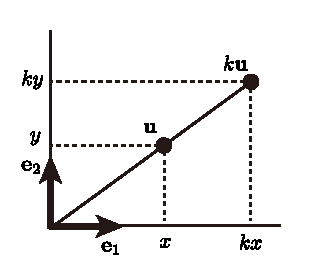
\includegraphics[width=1.0\linewidth]{/Users/kasa/Dropbox/GitHub/lectures/osaka-u/2023/kaenI/chap05_la/figures/la_vecscalar.eps}
\end{wrapfigure}
%
\Sec{row-column_vector}で述べたように,ベクトルは行列の1種である.
従って,行列の演算はそのままベクトルの演算の定義として使える.
ベクトルのスカラー倍とは,\Sec{mat_operation}にある通り,
%
\begin{align}
k\left[\begin{array}{c}
x\\
y
\end{array}\right] & =\left[\begin{array}{c}
kx\\
ky
\end{array}\right],
\end{align}
%
のような演算である.これはベクトルを,向きはそのままに長さを$k$倍に伸ばすということに対応している.
上式のスカラー倍は
%
\begin{align}
k\left[\begin{array}{c}
x\\
y
\end{array}\right] & =\left[\begin{array}{cc}
k & 0\\
0 & k
\end{array}\right]\left[\begin{array}{c}
x\\
y
\end{array}\right], 
\end{align}
とも書き直せる.つまり,ベクトルを伸ばすという操作は行列によって表すことができる.
右辺の対角行列のことをスカラー行列と呼ぶ.
%
\subsubsection{ベクトルの回転\label{sec:vec_rot}}
%

%
\begin{wrapfigure}{r}{5cm}
\centering
\vspace*{-\intextsep}
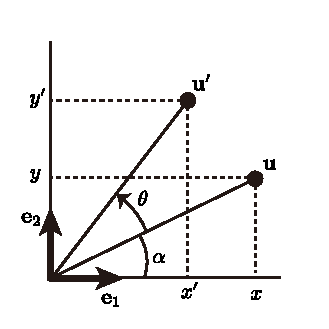
\includegraphics[width=1.0\linewidth]{/Users/kasa/Dropbox/GitHub/lectures/osaka-u/2023/kaenI/chap05_la/figures/la_plane.eps}  
\end{wrapfigure}
ここで,点P (位置ベクトル${\bf u}$, \Eq{LA:posvec})を原点Oを中心として時計回りに$\theta$回転させたベクトル${\bf u}^{\prime}$
%
\begin{align}
{\bf u}^{\prime} & =\left[\begin{array}{c}
x^{\prime}\\
y^{\prime}
\end{array}\right], 
\end{align}
%
がどう表されるかを見てみることにしよう.まず,元々のベクトル${\bf u}$を右図のように極座標表示
に直してみる.
%
\begin{align}
x & =r\cos\alpha,\\
y & =r\sin\alpha.
\end{align}
%
すると,回転後の各成分は加法定理を使って,次式のように表せることが分かる.
%
\begin{align}
x^{\prime} & =r\cos\left(\alpha+\theta\right)=r\cos\alpha\cos\theta-r\sin\alpha\sin\theta\notag\\
 & =x\cos\theta-y\sin\theta,\\
y^{\prime} & =r\sin\left(\alpha+\theta\right)=r\sin\alpha\cos\theta+r\cos\alpha\sin\theta\notag\\
 & =y\cos\theta+x\sin\theta.
\end{align}
%
これを行列表示に直すと,
%
\begin{align}
\left[\begin{array}{c}
x^{\prime}\\
y^{\prime}
\end{array}\right] & =\left[\begin{array}{cc}
\cos\theta & -\sin\theta\\
\sin\theta & \cos\theta
\end{array}\right]\left[\begin{array}{c}
x\\
y
\end{array}\right], \\
\rightarrow
{\bf u}^{\prime} & =\left[\begin{array}{cc}
\cos\theta & -\sin\theta\\
\sin\theta & \cos\theta
\end{array}\right]{\bf u}, 
\end{align}
%
となる.右辺の${\bf u}$にかかっている行列を回転行列と呼ぶ.
ここでは回転角$\theta$の回転行列を
\begin{align}
\hat{R}\left(\theta\right) & =\left[\begin{array}{cc}
\cos\theta & -\sin\theta\\
\sin\theta & \cos\theta
\end{array}\right], 
\end{align}
と表すことにする.
上式は,原点の周りの点(位置ベクトル${\bf a}$)の回転操作は,
${\bf a}$に行列をかけることで表せる.
また,ベクトル${\bf a}$を原点周りで$\theta$だけ回転させるという操作を$f_{\theta}\left({\bf a}\right)$と表すことにする.
\begin{align}
f_{\theta}\left({\bf a}\right) & = \hat{R}\left(\theta\right) {\bf a} 
=\left[\begin{array}{cc}
\cos\theta & -\sin\theta\\
\sin\theta & \cos\theta
\end{array}\right]{\bf a}. \label{LA:ftheta}
\end{align}
回転行列についてもう少し考察してみよう.\Eq{LA:uxe1ye2}の両辺に対して,回転操作$f_{\theta}$を行ってみる.
\begin{align}
f_{\theta}\left({\bf u}\right) & =f_{\theta}\left(x{\bf e}_{1}+y{\bf e}_{2}\right).
\end{align}
行列の積の性質\Eq{LA:matmult_parti}, \Eq{LA:matmul_scalar}から,$\hat{A}\left(\hat{B}+\hat{C}\right) = \hat{A}\hat{B} + \hat{A}\hat{C},~\hat{A}\left(k\hat{B}\right) = k\hat{A}\hat{B}$だから,上式は
\begin{align}
f_{\theta}\left({\bf u}\right) 
& = f_{\theta}\left(x{\bf e}_{1}\right) +  f_{\theta}\left(y{\bf e}_{2}\right)\notag\\
& = xf_{\theta}\left({\bf e}_{1}\right)+yf_{\theta}\left({\bf e}_{2}\right),
\end{align}
のように分解でき,さらに次のように行列表示
\begin{align}
f_{\theta}\left({\bf u}\right) & =
\left[\begin{array}{cc} f_{\theta}\left({\bf e}_{1}\right) & f_{\theta}\left({\bf e}_{2}\right)\end{array}\right]{\bf u}, \label{LA:ftheta_unitconv}
\end{align}
に直すことが出来る.上式と\Eq{LA:ftheta}との比較から,回転行列は$[\begin{array}{cc} f_{\theta}\left({\bf e}_{1}\right) & f_{\theta}\left({\bf e}_{2}\right)\end{array}]$,
つまり回転行列は基本ベクトル${\bf e}_{1},{\bf e}_{2}$を回転させたベクトル$f_{\theta}\left({\bf e}_{1}\right),~f_{\theta}\left({\bf e}_{2}\right)$を横に並べた行列,ということが分かった.
一応書いておくと,
\begin{align}
f_{\theta}\left({\bf e}_{1}\right) & =\left[\begin{array}{c}
\cos\theta\\
\sin\theta
\end{array}\right],\quad f_{\theta}\left({\bf e}_{2}\right)=\left[\begin{array}{c}
-\sin\theta\\
\cos\theta
\end{array}\right], 
\end{align}
%
なので,確かに\Eq{LA:ftheta}で示した回転行列と$[\begin{array}{cc} f_{\theta}\left({\bf e}_{1}\right) & f_{\theta}\left({\bf e}_{2}\right)\end{array}]$は一致する.

回転行列の逆行列について考えてみよう.
まず,原点周りに$-\theta$回転させる操作$f_{-\theta}\left({\bf a}\right)$は
\begin{align}
f_{-\theta}\left({\bf a}\right) & =\left[\begin{array}{cc}
\cos\left(-\theta\right) & -\sin\left(-\theta\right)\\
\sin\left(-\theta\right) & \cos\left(-\theta\right)
\end{array}\right]{\bf a}=\left[\begin{array}{cc}
\cos\theta & \sin\theta\\
-\sin\theta & \cos\theta
\end{array}\right]{\bf a}, \label{LA:f-theta}
\end{align}
%
である.\Eq{LA:f-theta}と\Eq{LA:ftheta}に現れる回転行列をかけると,
\begin{align}
\left[\begin{array}{cc}
\cos\theta & \sin\theta\\
-\sin\theta & \cos\theta
\end{array}\right] 
\left[\begin{array}{cc}
\cos\theta & -\sin\theta\\
\sin\theta & \cos\theta
\end{array}\right]
& =\left[\begin{array}{cc}
\cos^{2}\theta+\sin^{2}\theta & \cos\theta\sin\theta-\sin\theta\cos\theta\\
\sin\theta\cos\theta-\cos\theta\sin\theta & \sin^{2}\theta+\cos^{2}\theta
\end{array}\right]\notag\\
 & =\left[\begin{array}{cc}
1 & 0\\
0 & 1
\end{array}\right],
\end{align}
となるので,$\theta$回転させる回転行列の逆行列は$-\theta$回転させる回転行列であることが分かる (行列の積の順序を入れ替えた場合についても同様に対角行列になる.これは各自で確認しよう).
$\theta$回転させたものを$-\theta$回転させれば元に戻るので,考えてみれば自然なことではある.

次に,$\theta$回転させた後にさらに$\theta^{\prime}$回転させる操作を考える.
この操作を$f_{\theta^{\prime}}\circ f_{\theta}$と表すことにする.
これは一気に$\theta+\theta^{\prime}$回転させた操作$f_{\theta+\theta^{\prime}}$と同じになることが容易に想像される.このことが実際に正しいことを行列演算で確かめよう.
$f_{\theta+\theta^{\prime}}\left({\bf a}\right)$は
\begin{align}
f_{\theta+\theta^{\prime}}\left({\bf a}\right) & =\left[\begin{array}{cc}
\cos\left(\theta+\theta^{\prime}\right) & -\sin\left(\theta+\theta^{\prime}\right)\\
\sin\left(\theta+\theta^{\prime}\right) & \cos\left(\theta+\theta^{\prime}\right)
\end{array}\right]{\bf a},
\end{align}
%
であり,$f_{\theta^{\prime}}\circ f_{\theta}\left({\bf a}\right)$は
%
\begin{align}
f_{\theta^{\prime}}\circ f_{\theta}\left({\bf a}\right) & =\left[\begin{array}{cc}
\cos\theta^{\prime} & -\sin\theta^{\prime}\\
\sin\theta^{\prime} & \cos\theta^{\prime}
\end{array}\right]\left[\begin{array}{cc}
\cos\theta & -\sin\theta\\
\sin\theta & \cos\theta
\end{array}\right]{\bf a}, 
\end{align}
で表されるが,加法定理を用いることにより,
\begin{align}
f_{\theta^{\prime}}\circ f_{\theta}\left({\bf a}\right) & =\left[\begin{array}{cc}
\cos\theta^{\prime}\cos\theta-\sin\theta^{\prime}\sin\theta & -\cos\theta^{\prime}\sin\theta-\sin\theta^{\prime}\cos\theta\\
\sin\theta^{\prime}\cos\theta+\cos\theta^{\prime}\sin\theta & -\sin\theta^{\prime}\sin\theta+\cos\theta^{\prime}\cos\theta
\end{array}\right]{\bf a}\notag\\
 & =\left[\begin{array}{cc}
\cos\left(\theta+\theta^{\prime}\right) & -\sin\left(\theta+\theta^{\prime}\right)\\
\sin\left(\theta+\theta^{\prime}\right) & \cos\left(\theta+\theta^{\prime}\right)
\end{array}\right]{\bf a}\notag\\
 & =f_{\theta+\theta^{\prime}}\left({\bf a}\right), 
\end{align}
%
となり,$f_{\theta+\theta^{\prime}} = f_{\theta^{\prime}}\circ f_{\theta}$が示せた.
%
\subsection{1次変換(線形変換)}
%
ベクトル${\bf u}$を別のベクトル${\bf w}$に移す操作${\bf w}= f\left({\bf u}\right)$を考える.
$f$が次の条件を満たすとき,$f$を1次変換(線形変換)と呼ぶ.
%
\begin{align}
f\left(k{\bf u}\right) & =kf\left({\bf u}\right),\\
f\left({\bf u}+{\bf v}\right) & =f\left({\bf u}\right)+f\left({\bf v}\right),
\end{align}
%
\Eq{LA:matmul_scalar}と\Eq{LA:matmult_parti}を見て分かるように,
これらは行列の積が満たす性質でもある.つまり,
行列によって表されるベクトルの変換操作(スカラー倍や原点周りの回転)は1次変換である.

一次変換$f$
\begin{align}
 {\bf w} &= f\left({\bf u}\right)  =\hat{A}{\bf u},
\end{align}
について,行列$\hat{A}$が正則($\det(\hat{A}) \neq 0$),つまり逆行列$\hat{A}^{-1}$が存在する場合について考えてみる.
このとき,${\bf w}$を元の${\bf u}$に戻す1次変換$f^{-1}$が存在し,それは
\begin{align}
{\bf u} & =f^{-1}\left({\bf w}\right)=\hat{A}^{-1}{\bf w},
\end{align}
と表せる.というのも,上式の右辺は
\begin{align}
\hat{A}^{-1}{\bf w} & =\hat{A}^{-1}\left(\hat{A}{\bf u}\right)=\left(\hat{A}^{-1}\hat{A}\right){\bf u}\notag\\
 & ={\bf u},
\end{align}
となるからである.
全ての${\bf u}$に対して,${\bf w}=\hat{A}{\bf u}$の解${\bf u}=\hat{A}^{-1}{\bf w}$が存在し,
解はこれ以外に存在しない.また,全ての${\bf w}$に対して,${\bf u}=\hat{A}^{-1}{\bf w}$の唯一の解${\bf w}=\hat{A}{\bf u}$が存在する.
従って,$\hat{A}$に逆行列が存在するとき,1次変換で移されたベクトル${\bf w}$と移される前のベクトル${\bf u}$は1対1
に対応している.
%ここでいう1対1対応とは,${\bf u}_{1},~{\bf u}_{2}$が${\bf u}_{1}\neq {\bf u}_{2}$を満たすとき,

%そして,\Sec{vec_scalar}や\Sec{vec_rot}で示したように,
%ベクトルのスカラー倍や原点周りの回転といった操作は行列によって表せるので,
%これらは1次変換である.

%
\subsubsection{行列式の解釈}
%
%
\begin{wrapfigure}{r}{5cm}
  \centering
  \vspace*{-\intextsep}
  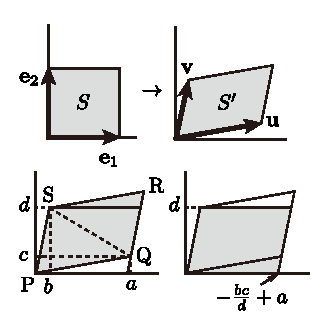
\includegraphics[width=1.0\linewidth]{/Users/kasa/Dropbox/GitHub/lectures/osaka-u/2023/kaenI/chap05_la/figures/la_det2d.eps} 
\end{wrapfigure}
%
基本ベクトル
%
\begin{align}
{\bf e}_{1} & =\left[\begin{array}{c}
1\\
0
\end{array}\right],\quad{\bf e}_{2}=\left[\begin{array}{c}
0\\
1
\end{array}\right], 
\end{align}
が張る正方形の面積を$S$とすると(右図左上),$S=1$である.
%
1次変換$f$
\begin{align}
f\left({\bf a}\right) & =\hat{A}{\bf a}\notag\\
 & =\left[\begin{array}{cc}
a & b\\
c & d
\end{array}\right]{\bf a}, 
\end{align}
を考える.ここでは$a,b,c,d$を実数とする.
一次変換$f$により基本ベクトル${\bf e}_{1},{\bf e}_{2}$はそれぞれ,
\begin{align}
{\bf u} & =f\left({\bf e}_{1}\right)
=
\left[\begin{array}{c}
a\\
c
\end{array}\right],\\
{\bf v} & =f\left({\bf e}_{2}\right)
=
\left[\begin{array}{c}
b\\
d
\end{array}\right],  
\end{align}
に移る.いま,${\bf u}$と${\bf v}$が向きの異なるベクトルだったとして,
${\bf u}, {\bf v}$が張る平行四辺形PQRSの面積$S^{\prime}$を求めてみる(上図右上と左下).
%
少し考えてみると分かるが,上図右下の平行四辺形の面積を求めても同じである(等積変形).
従って,点Q, Rを通る直線と$x$軸($y=0$)との交点が分かれば(つまり,底辺の長さが分かれば),直ちに面積が求まる.
この直線上の点$(x,y)$は変数$t$を用いて,
%
\begin{align}
\left[\begin{array}{c}
x\\
y
\end{array}\right] & =t{\bf v}+{\bf u}\notag\\
 & =\left[\begin{array}{c}
bt+a\\
dt+c
\end{array}\right], 
\end{align}
と表せる.$x$軸($y=0$)と交わるのは$t=-c/d$のときなので,
このとき$x=-(bc/d)+a$である.従って,面積$S^{\prime}$は
\begin{align}
S & =\left|d\times\left(-\dfrac{bc}{d}+a\right)\right|\notag\\
 & =\left|ad-bc\right|, 
\end{align}
となる.これは,\Sec{2d_invmat}で示した2次の正方行列$\hat{A}$の逆行列の絶対値をとったものに等しい.
\begin{align}
 S = \left|\det(\hat{A})\right|.
\end{align}
%
つまり,一次変換$f$により,長さ1の正方形が面積$\left|\det(\hat{A})\right|$の平行四辺形に変わるということが分かった.
これを一般化すると,二次元平面上の図形は1次変換により面積が$\det(\hat{A})$倍の図形に変わるということが示せる.

%
次に,$\det(\hat{A})$の符号について考えてみよう.
${\bf v}$を,時計回りに${\bf u}$に$\theta$ ($0<\theta < 2\pi$)だけ回転させて$k$倍($k>0$)したものとして表す.
\begin{align}
{\bf v} & =kf_{\theta}\left({\bf u}\right).
\end{align}
式変形していくと,
\begin{align}
{\bf v} & =kf_{\theta}\left({\bf u}\right)
 =k\hat{R}\left(\theta\right){\bf u}\notag\\
 & =k\left[\begin{array}{cc}
\cos\theta & -\sin\theta\\
\sin\theta & \cos\theta
\end{array}\right]\left[\begin{array}{c}
a\\
c
\end{array}\right]\notag\\
 & =k\left[\begin{array}{c}
a\cos\theta-c\sin\theta\\
a\sin\theta+c\cos\theta
\end{array}\right],
\end{align}
となる.これは行列$\hat{A}$を
\begin{align}
\hat{A} & =\left[\begin{array}{cc}
a & b\\
c & d
\end{array}\right]
 =\left[\begin{array}{cc}
a & k\left(a\cos\theta-c\sin\theta\right)\\
c & k\left(a\sin\theta+c\cos\theta\right)
\end{array}\right], 
\end{align}
と書き直したことに対応しており,行列式は
\begin{align}
\det(\hat{A}) & =\left|\begin{array}{cc}
a & k\left(a\cos\theta-c\sin\theta\right)\\
c & k\left(a\sin\theta+c\cos\theta\right)
\end{array}\right|\notag\\
 & =k\left(a^{2}+c^{2}\right)\sin\theta, 
\end{align}
となる.$a,c$は実数なので,行列式の正負は$\sin \theta$で決まる.
つまり,行列$\hat{A}$の1列目のベクトル${\bf u}$に対して,2列目のベクトル${\bf v}$が左側($0 <\theta < \pi$)にあるか右側($\pi < \theta < 2\pi$)にあるかで行列式の符号が決まる.
%
\subsubsection{行列式がゼロのときの1次変換\label{sec:linear_trans_det0_2d}}
%
上記の議論では,
${\bf u}$と${\bf v}$が異なる向きを持つベクトルであるとして,${\bf u}$と${\bf v}$が作る平行四辺形の面積について考えた.今度は,${\bf u}$と${\bf v}$が原点を通る同じ直線
上にあるときを考えてみよう.${\bf v}$は,
\begin{align}
 {\bf v} = k {\bf u}, 
\end{align}
と表せる.
このとき${\bf u}$と${\bf v}$が作る図形はつぶれてしまっていて,面積はゼロである.
実際,行列
\begin{align}
\hat{A} & =\left[\begin{array}{cc}
{\bf u} & k{\bf v}\end{array}\right]\notag\\
 & =\left[\begin{array}{cc}
a & ka\\
c & kc
\end{array}\right], 
\end{align}
の行列式$\det(\hat{A})$を計算してみるとゼロとなる.
では,この行列$\hat{A}$による一次変換はどのようなものだろうか?${\bf a}={}^{t}[\begin{array}{cc} p & q\end{array}]$として$\hat{A}{\bf a}$を計算してみよう.
すると,
\begin{align}
\hat{A}{\bf a} & =\left[\begin{array}{cc}
a & ka\\
c & kc
\end{array}\right]\left[\begin{array}{c}
p\\
q
\end{array}\right]=\left[\begin{array}{c}
ap+kaq\\
cp+kcq
\end{array}\right]
=\left(p+kq\right)\left[\begin{array}{c}
a\\
c
\end{array}\right] \notag \\
&= \left(p+kq\right){\bf u}, 
\end{align}
となる.
つまり,この1次変換によって,平面上のあらゆるベクトルは${\bf u}$のスカラー倍に変換される.
従って,${\bf a}$に関する方程式
\begin{align}
{\bf b} & =\hat{A}{\bf a}, \label{LA:b=Aa_det0}
\end{align}
は,${\bf b}$が${\bf u}$のスカラー倍のときのみ解が存在する
ということになるが,果たして解は1つだけだろうか?
実は上式を満たす${\bf a}$は無数に存在する.
そのことを以下で見ていこう.
まず,
\begin{align}
\hat{A}\bm{\omega} & ={\bf 0},
\end{align}
を満たす$\bm{\omega}$を考える($\bm{0}$は零ベクトル).これはすぐに見つけることができて,
\begin{align}
\bm{\omega}_{0} & =\left[\begin{array}{c}
k\\
-1
\end{array}\right], \label{LA:Aw=0} 
\end{align}
やこれのスカラー倍$t\bm{\omega}_{0}$が$\hat{A}\bm{\omega} = \bm{0}$を満たす\footnote{$\bm{\omega} = {}^{t}[\begin{array}{cc} r & s\end{array}]$などとおき,\Eq{LA:Aw=0}に代入して,$r,s$を求めれば良い.}.つまり,$\bm{\omega}_{0}$と同じ向きを持つベクトルは全て${\bf 0}$に移る.
\Eq{LA:b=Aa_det0}を満たす解の一つを${\bf a}_{0}$として見出したとして,
\begin{align}
 {\bf a} = {\bf a}_{0} + t \bm{\omega}_{0}, 
\end{align}
を考えると,
\begin{align}
\hat{A}\left({\bf a}_{0}+t\bm{\omega}_{0}\right)
&=\hat{A}{\bf a}_{0}+t\hat{A}\bm{\omega}_{0} \notag \\
& ={\bf b}+{\bf 0}={\bf b},
\end{align}
なので,\Eq{LA:b=Aa_det0}の解である.
$t$はどんな数でも良いので,\Eq{LA:b=Aa_det0}の解が無数に存在する.
従って,$\det(\hat{A})=0$のときには,変換前と変換後のベクトルの間の1対1対応が崩れてしまう.

少し脱線するが,自然科学への線形代数の応用を考える上で,
\begin{align}
 \hat{A}\bm{\omega} = \bm{0},
\end{align}
の形の方程式は重要である\footnote{主に量子力学のことを念頭に置いている.}.
$\det(\hat{A})\neq 0$のとき,上式を満たす$\bm{\omega}$は
\begin{align}
 \bm{\omega} = \hat{A}^{-1}\bm{0} = \bm{0}, 
\end{align}
の一つだけであるが,このテの方程式が自然科学の文脈で登場する場合,
$\bm{\omega}=\bm{0}$は物理的に意味のない解であることが多い.そこで,${\bf 0}$以外の解$\bm{\omega}$が存在しなければならない,という物理的要請が課されるわけだが,
この節での議論で既に見たように,
この要請は$\det(\hat{A}) = 0$として表せる\footnote{証明はしないが,$\det(\hat{A})=0$であることと,$\hat{A}\bm{\omega}=\bm{0}$を満たす$\bm{\omega}$が${\bm 0}$以外に存在することは同値である.}.
$\det(\hat{A})=0$という関係式が得られると何が嬉しいかというと,例えば,$\hat{A}$が既知の数$a,b$と未知数$x$からなる
\begin{align}
\hat{A} & =\left[\begin{array}{cc}
a-x & b-x\\
b-x & a-x
\end{array}\right], 
\end{align}
のような形の行列だったとすると,$\det(\hat{A})=0$から,
\begin{align}
 \det(\hat{A}) & =\left(a-x\right)^{2}-\left(b-x\right)^{2}=0,
\end{align}
のように,$x$に関する方程式が得られるという点にある.
$\det(\hat{A})=0$から得られる方程式のことを永年方程式と呼ぶ.
%
\subsection{行列式の性質}
%
行列式が持つ性質についていくつか紹介する.
なお,ここで示した性質は$n$次の正方行列についても成り立つ\footnote{$n$次の正方行列について議論する際に改めて述べる.}.
%
\subsubsection{$\det(\hat{A}\hat{B}) = \det(\hat{A})\det(\hat{B})$}
%
正方行列$\hat{A}$と$\hat{B}$について次式が成り立つ.
%
\begin{align}
  \det(\hat{A}\hat{B}) & = \det(\hat{A}) \det(\hat{B}). \label{LA:det(AB)=det(A)det(B)_2D}
\end{align}
%
これを2次の正方行列の場合に示しておく.
$\hat{A}$と$\hat{B}$を
%
\begin{align}
\hat{A} & =\left[\begin{array}{cc}
a_{11} & a_{12}\\
a_{21} & a_{22}
\end{array}\right],\quad\hat{B}=\left[\begin{array}{cc}
b_{11} & b_{12}\\
b_{21} & b_{22}
\end{array}\right],
\end{align}
%
と定義すると,それぞれの行列式は
%
\begin{align}
\det(\hat{A}) & =a_{11}a_{22}-a_{12}a_{21},\\
\det(\hat{B}) & =b_{11}b_{22}-b_{12}b_{21}, 
\end{align}
%
であるから,
%
\begin{align}
\det(\hat{A})\det(\hat{B}) & =\left(a_{11}a_{22}-a_{12}a_{21}\right)\left(b_{11}b_{22}-b_{12}b_{21}\right)\notag\\
 & =a_{11}a_{22}\left(b_{11}b_{22}-b_{12}b_{21}\right)-a_{12}a_{21}\left(b_{11}b_{22}-b_{12}b_{21}\right).
\end{align}
%
次に,$\hat{A}\hat{B}$は,
%
\begin{align}
\hat{A}\hat{B} & =\left[
\begin{array}{cc}
a_{11}b_{11}+a_{12}b_{21} & a_{11}b_{12}+a_{12}b_{22}\\
a_{21}b_{11}+a_{22}b_{21} & a_{21}b_{12}+a_{22}b_{22}
\end{array}
\right], 
\end{align}
%
なので,$\det(\hat{A}\hat{B})$は愚直に計算すると,
\begin{align}
\det(\hat{A}\hat{B}) & =\left(a_{11}b_{11}+a_{12}b_{21}\right)\left(a_{21}b_{12}+a_{22}b_{22}\right)-\left(a_{11}b_{12}+a_{12}b_{22}\right)\left(a_{21}b_{11}+a_{22}b_{21}\right)\notag\\
 & =a_{11}a_{21}b_{11}b_{12}+a_{11}a_{22}b_{11}b_{22}+a_{12}a_{21}b_{21}b_{12}+a_{11}a_{22}b_{21}b_{22}\notag\\
 & \quad-a_{11}a_{21}b_{12}b_{11}-a_{11}a_{22}b_{12}b_{21}-a_{12}a_{21}b_{22}b_{11}-a_{12}a_{22}b_{22}b_{21}\notag\\
 & =a_{11}a_{22}b_{11}b_{22}+a_{12}a_{21}b_{21}b_{12}-a_{11}a_{22}b_{12}b_{21}-a_{12}a_{21}b_{22}b_{11}\notag\\
 & =a_{11}a_{22}\left(b_{11}b_{22}-b_{12}b_{21}\right)-a_{12}a_{21}\left(b_{11}b_{22}-b_{21}b_{12}\right).
\end{align}
%
従って,\Eq{LA:det(AB)=det(A)det(B)_2D}が成り立つことが示せた.
%
\subsubsection{$\det({}^{t}\hat{A})=\det(\hat{A})$}
%
正方行列$\hat{A}$の行列式$\det(\hat{A})$と転置行列${}^{t}\hat{A}$の行列式$\det({}^{t}\hat{A})$は等しい.
%
\begin{align}
\det({}^{t}\hat{A})=\det(\hat{A}). \label{LA:det(tA)=det(A)_2D}
\end{align}
%
これを2次の正方行列の場合に示す.$\hat{A}$を
%
\begin{align}
\hat{A} & =\left[\begin{array}{cc}
a_{11} & a_{12}\\
a_{21} & a_{22}
\end{array}\right], 
\end{align}
%
と定義すると,${}^{t}\hat{A}$は
%
\begin{align}
{}^{t}\hat{A} & =\left[\begin{array}{cc}
a_{11} & a_{21}\\
a_{12} & a_{22}
\end{array}\right], 
\end{align}
%
である.それぞれの行列式を計算すると,
\begin{align}
\det(\hat{A}) & =a_{11}a_{22}-a_{12}a_{21},\\
\det({}^{t}\hat{A}) & =a_{11}a_{22}-a_{21}a_{12},
\end{align}
%
なので,\Eq{LA:det(tA)=det(A)_2D}が示せた.
%
\subsection{基底と座標変換}
%
\begin{wrapfigure}{r}{5cm}
  \centering
  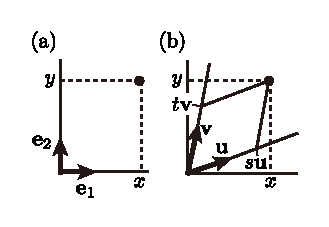
\includegraphics[width=1.0\linewidth]{figures/la_basis_e1e2.eps} 
\end{wrapfigure}

これまで,平面上の点(位置ベクトル) ${\bf a}$を表すために,
互いに直交する基本ベクトル${\bf e}_{1},{\bf e}_{2}$を決めて,
\begin{align}
{\bf a} & =x{\bf e}_{1}+y{\bf e}_{2}, \label{a=xe1+ye2_2D}
\end{align}
のような形で表していた(右図(a)).
これは,${\bf e}_{1},{\bf e}_{2}$を使った位置の表現であるが,
別のベクトルの組${\bf u},{\bf v}$を「適切に」選べば,
%
\begin{align}
{\bf a} & =s{\bf u}+t{\bf v}, \label{LA:a=su+tv_basis}
\end{align}
%
のような別の表現もできるはずだ(右図(b)).
この「適切な」ベクトルの組とはどのようなものを指すかを考えてみる.
平面上の全ての点を\Eq{LA:a=su+tv_basis}の形で表せないと困るので,
この要請を満たす${\bf u},{\bf v}$を適切なベクトルの組と定義しよう.
${\bf u}$と${\bf v}$が平行できないとき,この要請を満たすが,
${\bf u}$と${\bf v}$が平行のとき(${\bf v}=k{\bf u}$)は
直線$t{\bf u}$上の点しか表せない.
従って,\Sec{linear_trans_det0_2d}での議論から,適切なベクトルの組は
\begin{align}
\det\left(\left[\begin{array}{cc}
{\bf u} & {\bf v}\end{array}\right]\right) & \neq0, \label{LA:detA0_basis_2D}
\end{align}
を満たすものである.この条件を満たすベクトルの組${\bf u},{\bf v}$を数学では基底と呼ぶ.
行列式がゼロでないとき,
\begin{align}
s{\bf u}+t{\bf v} & =\left[\begin{array}{cc}
{\bf u} & {\bf v}\end{array}\right]\left[\begin{array}{c}
s\\
t
\end{array}\right]={\bf 0},
\end{align}
を満たす$s,t$は$s=t=0$以外にない(
$[\begin{array}{cc}
{\bf u} & {\bf v}\end{array}]$の逆行列が存在するため).
これは特定の点を表現するための$s,t$は1通りしかないことを意味している.
なぜなら,
%
\begin{align}
{\bf a} & =s{\bf u}+t{\bf v}=s^{\prime}{\bf u}+t^{\prime}{\bf v},
\end{align}
の2通りの表現を考えたとして,式変形すると,
\begin{align}
\left(s-s^{\prime}\right){\bf u}+\left(t-t^{\prime}\right){\bf v} & ={\bf 0},
\end{align}
であることから,結局\Eq{LA:detA0_basis_2D}より$s=s^{\prime},t=t^{\prime}$が導かれるためである.
逆に点${\bf a}$を表す$s,t$が1通りであるとき,方程式
\begin{align}
\left[\begin{array}{cc}
{\bf u} & {\bf v}\end{array}\right]\left[\begin{array}{c}
s\\
t
\end{array}\right] & ={\bf a}, 
\end{align}
が唯一の解$s,t$を持つということだから,
\begin{align}
\left[\begin{array}{c}
s\\
t
\end{array}\right] & =\left[\begin{array}{cc}
{\bf u} & {\bf v}\end{array}\right]^{-1}{\bf a},
\end{align}
のように逆行列が存在せねばならないので,その行列式はゼロである.
従って,ベクトル${\bf u},{\bf v}$の組が作る行列の行列式がゼロでないことと,$s,t$が1通りで決まることは同値である.

基底${\bf u},{\bf v}$を使って,ベクトル${\bf a}$を
\begin{align}
{\bf a} & =s{\bf u}+t{\bf v}, 
\end{align}
のように表すことを,${\bf u}$と${\bf v}$の1次結合(線形結合)と呼ぶ.\Eq{a=xe1+ye2_2D}と上式を組み合わせると,
\begin{align}
\left[\begin{array}{c}
x\\
y
\end{array}\right] & =\left[\begin{array}{cc}
{\bf u} & {\bf v}\end{array}\right]\left[\begin{array}{c}
s\\
t
\end{array}\right], 
\end{align}
と表せる.左辺の$x,y$は${\bf e}_{1},{\bf e}_{2}$を基底としたときの座標,
右辺の$s,t$は${\bf u},{\bf v}$を基底としたときの座標である.
上式は2つの異なる基底を関係付ける式であり,$s,t$から$x,y$を求めるときは上式を使い,
$x,y$から$s,t$を求めるときには,
\begin{align}
\left[\begin{array}{c}
s\\
t
\end{array}\right] & =\left[\begin{array}{cc}
{\bf u} & {\bf v}\end{array}\right]^{-1}\left[\begin{array}{c}
x\\
y
\end{array}\right], \label{LA:coordinate_transform_2D}
\end{align}
を使うことになる.このように座標系をとりかえることを座標変換と呼ぶ.
%
\subsubsection{行列の座標変換}
%
基底${\bf u}_{1},{\bf u}_{2}$を用意して,基本ベクトル${\bf e}_{1},{\bf e}_{2}$で座標が$(x,y)$と表される点を
\begin{align}
\left[\begin{array}{c}
x\\
y
\end{array}\right] & =\left[\begin{array}{cc}
{\bf u}_{1} & {\bf u}_{2}\end{array}\right]\left[\begin{array}{c}
s\\
t
\end{array}\right],
\end{align}
と表したとする.$(s,t)$は基底${\bf u}_{1},{\bf u}_2$上の点の座標である.
上式に対して,行列$\hat{A}$で表される1次変換
%
\begin{align}
\left[\begin{array}{c}
x^{\prime}\\
y^{\prime}
\end{array}\right] 
& =f\left(\left[\begin{array}{c}
x\\
y
\end{array}\right]\right)=\hat{A}\left[\begin{array}{c}
x\\
y
\end{array}\right],
\end{align}
%
を作用させると,
%
\begin{align}
\left[\begin{array}{c}
x^{\prime}\\
y^{\prime}
\end{array}\right] & =\hat{A}\left[\begin{array}{cc}
{\bf u}_{1} & {\bf u}_{2}\end{array}\right]\left[\begin{array}{c}
s\\
t
\end{array}\right],
\end{align}
が得られるが,これは基底${\bf u}_{1},{\bf u}_{2}$上の座標$(s,t)$が
1次変換により,基底${\bf e}_{1},{\bf e}_{2}$上の座標$(x^{\prime},y^{\prime})$
にうつったことを意味する.1次変換後の座標も基底${\bf u}_{1},{\bf u}_{2}$上でのものを知りたい場合は,
得られたベクトル
$[\begin{array}{cc}
x^{\prime} &
y^{\prime}
\end{array}]$ 
を${\bf u}_{1},{\bf u}_{2}$を用いて
%
\begin{align}
\left[\begin{array}{c}
x^{\prime}\\
y^{\prime}
\end{array}\right] & =\left[\begin{array}{cc}
{\bf u}_{1} & {\bf u}_{2}\end{array}\right]\left[\begin{array}{c}
s^{\prime}\\
t^{\prime}
\end{array}\right],
\end{align}
と表せば,座標変換の式(\Eq{LA:coordinate_transform_2D})から,
%
\begin{align}
\left[\begin{array}{c}
s^{\prime}\\
t^{\prime}
\end{array}\right] & =\left[\begin{array}{cc}
{\bf u}_{1} & {\bf u}_{2}\end{array}\right]^{-1}\left[\begin{array}{c}
x^{\prime}\\
y^{\prime}
\end{array}\right]\notag\\
 & =\left[\begin{array}{cc}
{\bf u}_{1} & {\bf u}_{2}\end{array}\right]^{-1}\hat{A}\left[\begin{array}{cc}
{\bf u}_{1} & {\bf u}_{2}\end{array}\right]\left[\begin{array}{c}
s\\
t
\end{array}\right]
\end{align}
のように,同じ基底上で,1次変換により座標がどのように変化するかを知ることができる.
%
%
\subsection{行列の対角化}
%
\begin{align}
\hat{B} & =\left[\begin{array}{cc}
{\bf u}_{1} & {\bf u}_{2}\end{array}\right]^{-1}\hat{A}\left[\begin{array}{cc}
{\bf u}_{1} & {\bf u}_{2}\end{array}\right], 
\end{align}
%
\subsubsection{固有ベクトルと固有値}
%
ベクトル${\bf u}$に対して2次の正方行列$\hat{A}$で表される1次変換を行なったときに,
${\bf u}$のスカラー倍になる,つまり
%
\begin{align}
\hat{A}{\bf u} & =\lambda{\bf u}, \label{LA:eigen_equation_2D} 
\end{align}
%
が成り立つとき,${\bf u}$を$\hat{A}$の固有ベクトル,$\lambda$のことを固有値と呼ぶ.
\Eq{LA:eigen_equation_2D}を満たす${\bf u}$が2つ得られたとして,
そのベクトルを${\bf u}_{1},{\bf u}_{2}$とおくことにする.
また,${\bf u}_{1},{\bf u}_{2}$の固有値をそれぞれ$\lambda,\mu~(\lambda \neq \mu)$とする.
%
${\bf u}_{1},{\bf u}_{2}$の線形結合
%
\begin{align}
{\bf u} & =s{\bf u}_{1}+t{\bf u}_{2},
\end{align}
%
を考えると,\Eq{LA:eigen_equation_2D}より,
%
\begin{align}
\hat{A}{\bf u} & =\hat{A}\left(s{\bf u}_{1}+t{\bf u}_{2}\right)=s\hat{A}{\bf u}_{1}+t\hat{A}{\bf u}_{2}\notag\\
 & =s\lambda{\bf u}_{1}+t\mu{\bf u}_{2}\notag\\
 & =\left[\begin{array}{cc}
{\bf u}_{1} & {\bf u}_{2}\end{array}\right]\left[\begin{array}{c}
s\lambda\\
t\mu
\end{array}\right],
\end{align}
となるが,左辺を少し眺めると,スカラー行列を使ってさらに
\begin{align}
\left[\begin{array}{cc}
{\bf u}_{1} & {\bf u}_{2}\end{array}\right]\left[\begin{array}{c}
s\lambda\\
t\mu
\end{array}\right] & =\left[\begin{array}{cc}
{\bf u}_{1} & {\bf u}_{2}\end{array}\right]\left[\begin{array}{cc}
\lambda & 0\\
0 & \mu
\end{array}\right]\left[\begin{array}{c}
s\\
t
\end{array}\right],
\end{align}
%
と式変形出来ることがわかる.
%
$\hat{A}\left(s{\bf u}_{1}+t{\bf u}_2\right)$は
\begin{align}
\hat{A}\left(s{\bf u}_{1}+t{\bf u}_{2}\right) & =\hat{A}\left[\begin{array}{cc}
{\bf u}_{1} & {\bf u}_{2}\end{array}\right]\left[\begin{array}{c}
s\\
t
\end{array}\right], 
\end{align}
%
と書き直せるので,
\begin{align}
\hat{A}\left[\begin{array}{cc}
{\bf u}_{1} & {\bf u}_{2}\end{array}\right] & \left[\begin{array}{c}
s\\
t
\end{array}\right]=\left[\begin{array}{cc}
{\bf u}_{1} & {\bf u}_{2}\end{array}\right]\left[\begin{array}{cc}
\lambda & 0\\
0 & \mu
\end{array}\right]\left[
\begin{array}{c}
s\\
t
\end{array}
\right],
\end{align}
である.$s,t$については何も指定していなかったので,
${}^{t}[
\begin{array}{cc}
s & t \\
\end{array}
]$
%
の係数部分を取り出すことで,次式が得られる.
%
\begin{align}
\hat{A}\left[\begin{array}{cc}
{\bf u}_{1} & {\bf u}_{2}\end{array}\right] & =\left[\begin{array}{cc}
{\bf u}_{1} & {\bf u}_{2}\end{array}\right]\left[\begin{array}{cc}
\lambda & 0\\
0 & \mu
\end{array}\right]. 
\end{align}
%
両辺に左から$[
\begin{array}{cc}
{\bf u}_{1} & {\bf u}_{2} \\
\end{array}
]^{-1}$をかけることで,
%
\begin{align}
\left[\begin{array}{cc}
{\bf u}_{1} & {\bf u}_{2}\end{array}\right]^{-1}\hat{A}\left[\begin{array}{cc}
{\bf u}_{1} & {\bf u}_{2}\end{array}\right] & =\left[\begin{array}{cc}
\lambda & 0\\
0 & \mu
\end{array}\right], 
\end{align}
が得られる.これは$\hat{A}$が対角化できたことを意味している.
つまり,$\hat{A}$を対角化するような基底は,
$\hat{A}$に対する固有ベクトルの組であるということが分かった.
%

上の式変形では
$[
\begin{array}{cc}
 {\bf u}_{1} & {\bf u}_{2} \\
\end{array}
]$
の逆行列が存在すると考えて進めていた.
ここからは,逆行列が存在することを示そう.
固有ベクトル${\bf u}_{1}$と${\bf u}_{2}$の固有値が異なっていれば,
%固有ベクトルを2つ求めて,それを横に並べた行列
%\begin{align}
%\hat{U} =
%\left[
%\begin{array}{cc}
%{\bf u}_{1} & {\bf u}_{2} 
%\end{array}
%\right],
%\end{align}
